\documentclass{beamer}
\usepackage[utf8]{inputenc}
% \usepackage{beamerthemesplit}
\setbeamertemplate{footline}[frame number]
\setbeamertemplate{navigation symbols}{}

\newcommand{\backupbegin}{
   \newcounter{finalframe}
   \setcounter{finalframe}{\value{framenumber}}
}
\newcommand{\backupend}{
   \setcounter{framenumber}{\value{finalframe}}
}


\title{Using Graph Neural Networks in Local Search for Edge-Based Relaxations of the Maximum Clique Problem}
\subtitle{Diploma Thesis - Logic and Computation}
\author{Rupert Ettrich \and \\ \scriptsize Advisors:  Ao.Univ.Prof. Dipl.-Ing. Dr.techn. Günther Raidl \and \\ Projektass. Marc Huber, MSc \\ Institute of Logic and Computation - Algorithms and Complexity Group}
\date{10 Jan 2023}

\begin{document}

\maketitle

% \begin{frame}{Outline}
% \begin{itemize}
%     \item Motivation and Aim of the Thesis
%     % \item Aim of the Thesis and Expected Results
%     \item State-of-the-Art
%     \item Methodology
%     \item Context within the Logic and Computation Master's Program
% \end{itemize}
    
% \end{frame}

\begin{frame}{Motivation and Aim of the Thesis}
    \begin{itemize}
        \item<1-> Combinatorial Optimization Problems (COPs): structured instances (graphs)
        \item<2-> Machine Learning (ML) in algorithms for COPs
        \item<3-> Graph Neural Networks (GNNs): NNs specifically tailored to learn from graph input 
    \end{itemize}
\begin{figure}
    \centering
    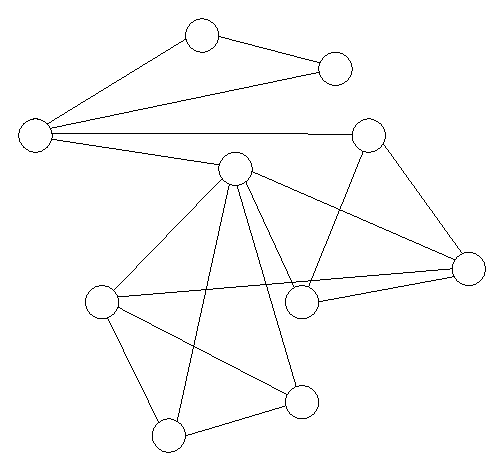
\includegraphics[width=0.3\textwidth]{graphics/graph1.eps}
\end{figure}
\end{frame}

\begin{frame}{Motivation and Aim of the Thesis}
    \begin{itemize}
        % \item<1-> End-to-end ML approaches not competitive to leading heuristic methods
        % \item<2-> Successful applications: e.g. GNN guided destroy operator in LNS \cite{Oberweger2022}
        \item<1-> Application of GNNs in context of (meta-)heuristics for COPs on graphs (MCP relaxations)
        \item<2-> For MCP relaxations: Most state-of-the-art heuristic algorithms based on local search
        \item<3-> Improve local search-based metaheuristic by utilizing GNN
        % \item<3-> Explore suitable GNN architectures
        % \item<4-> New heuristic solution for considered problems
    \end{itemize}
\end{frame}

\begin{frame}{Maximum Clique Problem}
    Given a graph $G = (V,E)$, find clique of maximum size in $G$
    \begin{itemize}
        % \item Decision variant is one of Karp's 21 NP-Complete problems \cite{Karp1972}
        % \item Applications in bioinformatics \cite{Dognin2010}, social network analysis \cite{Pattillo_network_analysis_2013}, etc...
        \item MCP too strict a model for many real-world applications
    \end{itemize}
    \begin{figure}
        \centering
        \includegraphics[width=0.3\textwidth]{graphics/graph1-clique.eps}
    \end{figure}
\end{frame} 

\begin{frame}{Maximum Quasi-Clique Problem}
    Given a graph $G = (V,E)$ and $\gamma \in (0,1]$, find $S \subseteq V$ of maximum size with edge density at least $\gamma$ in $G[S]$
    \begin{itemize}
        % \item<1-> Introduced in \cite{Abello2002}
        % \item<2-> Not hereditary - if $S$ is a $\gamma$-quasi clique, $S^\prime \subset S$ is not necessarily a $\gamma$-quasi clique
        \item<1-> Applications in bioinformatics, social network analysis, etc...
        \item<2-> NP-hard for $\gamma \in (0,1]$ \cite{pattillo_maximum_2013}
    \end{itemize}
    % \begin{figure}
    %     \centering
    %     \includegraphics[width=0.3\textwidth]{graphics/graph1-clique.eps}
    % \end{figure}
\end{frame}

\begin{frame}{State of the Art - Algorithms for MQCP}
    \begin{itemize}
        \item<1-> Exact methods: B\&B, MI(L)P, runtimes $> 1$ hour for dense instances with $|V|=100$
        % \begin{itemize}
        %     \item Most approaches either branch-and-bound or MI(L)P-formulations
        %     \item Leading methods fail to solve very dense graphs with 100 nodes in $<$ 1 hour
        % \end{itemize}
        \item<2-> Leading heuristic methods:
        \begin{itemize}
            \item<3-> Tabu Search \cite{djeddi_extension_2019}
            \item<4-> Memetic Algorithm (uses Tabu Search) \cite{zhou_opposition-based_2020}
            \item<5-> Local Search with Configuration Checking \cite{chen_nuqclq_2021}
            \item<6-> Hybrid Artificial Bee Colony Optimization (uses Tabu Search) \cite{peng_solving_2021}
        \end{itemize}
    \end{itemize}
\end{frame}

\begin{frame}{The Algorithm LSBM}
    \begin{itemize}
        \item Example: Search for Maximum Quasi Clique (MQC) with density $\gamma=0.9$ \\
        \item Approximate MQC by finding series of QCs of increasing size
    \end{itemize}
    \begin{figure}
        \centering
        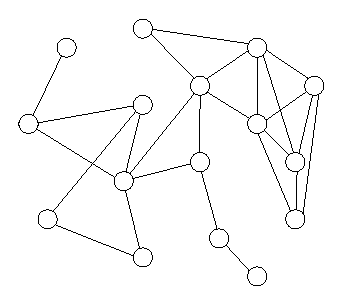
\includegraphics[width=0.6\textwidth]{graphics/algorithm_poster_0.eps}
    \end{figure}
\end{frame}

\begin{frame}{The Algorithm LSBM}
    \begin{itemize}
        \item Initially, Beam Search-based lower bound heuristic computes starting solution $S^*$ \\
    \end{itemize}
    \begin{figure}
        \centering
        \includegraphics[width=0.6\textwidth]{graphics/algorithm_poster_1.eps}
    \end{figure}
\end{frame}

\begin{frame}{The Algorithm LSBM}
    \begin{itemize}
        \item Construction heuristic computes candidate solution of size $|S^*|+1$
        \item Not a feasible 0.9-quasi clique yet - density is $\frac{7}{10}$
    \end{itemize}
    \begin{figure}
        \centering
        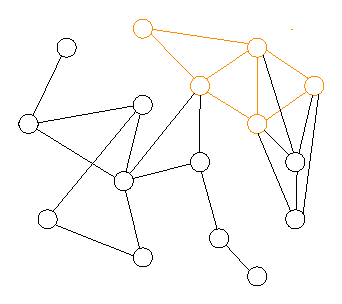
\includegraphics[width=0.6\textwidth]{graphics/algorithm_poster_2.eps}
    \end{figure}
\end{frame}

\begin{frame}{The Algorithm LSBM}
    \begin{itemize}
        \item Scoring function evaluates vertices in $G = (V, E)$
        \item Move operator: Swap vertex in candidate solution $S$ with vertex in $V \setminus S$
    \end{itemize}
    \begin{figure}
        \centering
        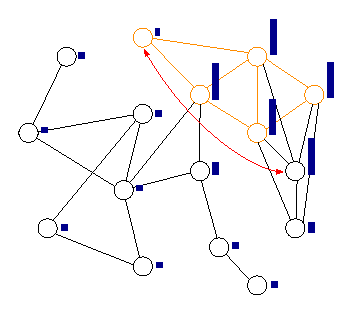
\includegraphics[width=0.6\textwidth]{graphics/algorithm_poster_3.eps}
    \end{figure}
\end{frame}

\begin{frame}{The Algorithm LSBM}
    \begin{itemize}
        \item Scoring function evaluates vertices in $G = (V, E)$
        \item Move operator: Swap vertex in candidate solution $S$ with vertex in $V \setminus S$
    \end{itemize}
    \begin{figure}
        \centering
        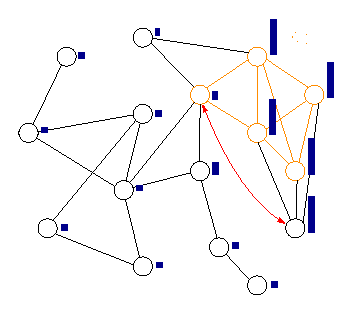
\includegraphics[width=0.6\textwidth]{graphics/algorithm_poster_4.eps}
    \end{figure}
\end{frame}

\begin{frame}{The Algorithm LSBM}
    \begin{itemize}
        \item<1-> Feasible QC of size 5 found
        \item<2-> Restart search for QC of size 6
        \item<3-> After a user-defined number of swaps without improvement, restart search
        \item<4-> After a user-defined number of restarts, return best found solution
        % \item<5-> Short-Term Memory: Tabu List
    \end{itemize}
    \begin{figure}
        \centering
        \includegraphics[width=0.5\textwidth]{graphics/algorithm_poster_6.eps}
    \end{figure}
\end{frame}

\begin{frame}{The scoring function $d_S$}
    \begin{itemize}
        \item Commonly used scoring function
        \item $d_S(v) = | S \cap N_G(v) |$
    \end{itemize}
    \begin{figure}
        \centering
        \includegraphics[width=0.6\textwidth]{graphics/ds1.eps}
    \end{figure}
\end{frame}

\begin{frame}{The scoring function $d_S$}
    Problems using $d_S$:
    \begin{itemize}
        \item<1-> Search gets stuck in local optima easily
        \item<2-> Many vertices have same $d_S$ value - how to break ties?
    \end{itemize}
\end{frame}

\begin{frame}{A GNN-based Metaheuristic}
    \begin{itemize}
        \item<1-> Use GNN-based scoring function $g_S$ to restrict neighborhood
        \item<2-> Take into account structural information as well as $d_S$-values
        \item<3-> Train GNN to imitate search of larger neighborhood
    \end{itemize}
\end{frame}

\begin{frame}{LSBM-T: Overview}
    \begin{itemize}
        \item<1-> Train $g_S$ offline on representative instances
        \item<2-> Imitate expert strategy that searches user-defined neighborhood structure
        \item<3-> Train $g_S$ in binary vertex classification task
        \item<4-> Training sample: $G, S$ + target values
    \end{itemize}
    \begin{figure}
        \centering
        \includegraphics[width=0.8\textwidth]{graphics/target_values.eps}<4->
    \end{figure}
\end{frame}

\begin{frame}{LSBM-T: Overview}
    \begin{figure}
        \centering
        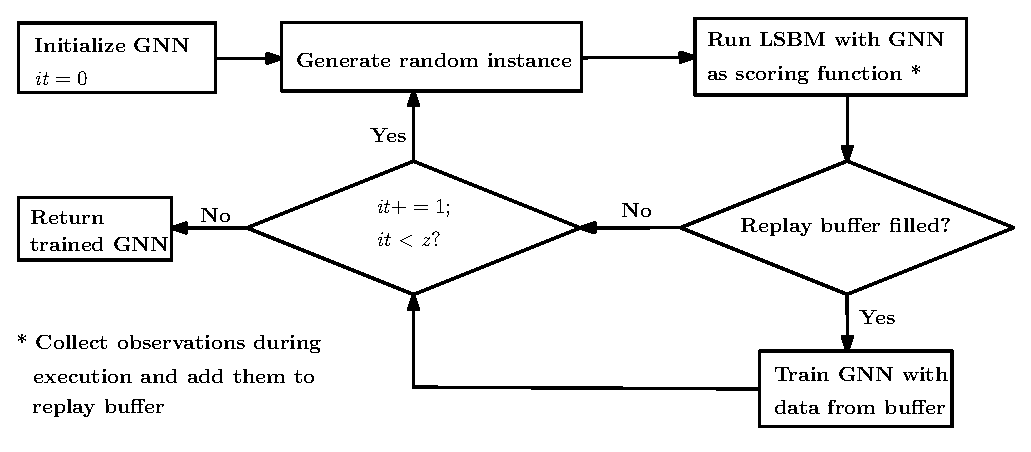
\includegraphics[width=\textwidth]{graphics/flowchart.eps}
    \end{figure}
\end{frame}

\begin{frame}{GNN - Evaluation}
    \begin{itemize}
        \item<1-> Once per graph: Initialize node features, compute embeddings
        \item<2-> After every swap: Compute context, apply Decoder
        \item<3-> Outputs: scores $\in [0,1]$
        \item<4-> Restrict neighborhood: Consider up to $k^\prime$ vertices in $S$ and $V \setminus S$
    \end{itemize}
    \begin{figure}
        \centering
        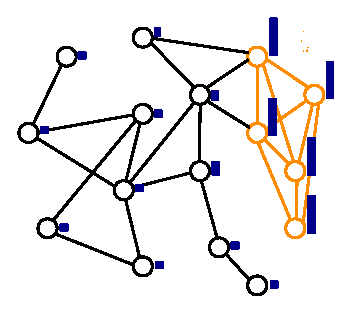
\includegraphics[width=0.5\textwidth]{graphics/algorithm_poster_5.eps}
    \end{figure}
\end{frame}

\begin{frame}{Feature Initialization}
    \begin{itemize}
        \item<1-> Non-attributed graphs
        \item<2-> Centrality-based initialization: Degree, EgoNet
        \item<3-> Learning-based initialization: Node2Vec \cite{GroverL16}, Struc2Vec \cite{FigueiredoRS17}
    \end{itemize}
    \begin{figure}
        \centering
        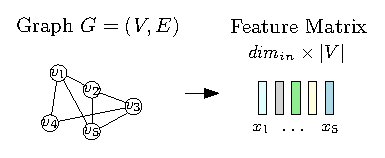
\includegraphics[width=0.7\textwidth]{graphics/architecture-1.eps}
    \end{figure}
\end{frame}

\begin{frame}{GNN Architecture}
    \begin{itemize}
        \item Attention-based Encoder based on \cite{Kool2019}
        \item Replace multi-head attention layers by newer GATv2 \cite{Brody2021} 
        \item Use GNN to create node embeddings, $O(n^2)$ once per graph
    \end{itemize}
    \begin{figure}
        \centering
        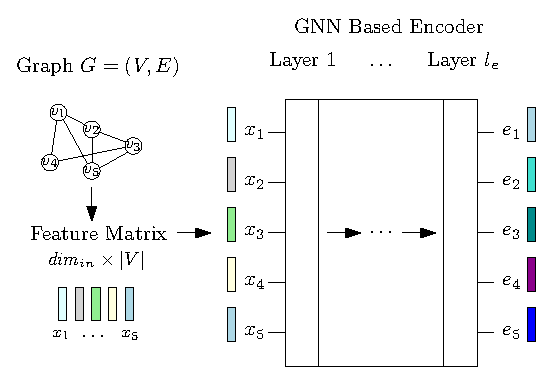
\includegraphics[width=0.7\textwidth]{graphics/architecture-2.eps}
    \end{figure}
\end{frame}

\begin{frame}{GNN Architecture}
    \begin{itemize}
        \item Context embedding: aggregate embeddings of vertices in $S$
        \item Add $d_S$-values, mean, std to context
    \end{itemize}
    \begin{figure}
        \centering
        \includegraphics[width=0.7\textwidth]{graphics/architecture-3.eps}
    \end{figure}
\end{frame}

\begin{frame}{GNN Architecture}
    \begin{itemize}
        \item Decoder: MLP with $\sigma$ activation, $O(n)$
    \end{itemize}
    \begin{figure}
        \centering
        \includegraphics[width=\textwidth]{graphics/architecture-4.eps}
    \end{figure}
\end{frame}

\begin{frame}{Results and Conclusions}
    \begin{itemize}
        \item<1-> GNN-based algorithm LSBM and training algorithm LSBM-T
        \item<2-> Attention-based Encoder-Decoder GNN architecture based on \cite{Kool2019}
        \item<3-> Analysis of computational overhead introduced by GNN
        \item<4-> LSBM-T successfully trains GNN to imitate exhaustive search of a neighborhood
        % \item<5-> Successful application of learning-based feature initialization methods
        \item<5-> Benchmark instances
        \item<6-> GNN-based scoring function outperforms $d_S$ on random graphs
    \end{itemize}
\end{frame}

\begin{frame}{Future Work}
    \begin{itemize}
        \item<1-> Improve generalization to larger instances
        \item<2-> Define stronger context that is independent of $d_S$
        \item<3-> Improve GNN: Two scores for each vertex
        \item<4-> Investigate GPU speedup
        \item<5-> Training data generation: Real-world datasets, other random graph models
    \end{itemize}
\end{frame}

\backupbegin

\bibliographystyle{apalike} 
\bibliography{final-presentation}

\begin{frame}{State of the Art - GNNs in COPs}
    \begin{itemize}
        \item<1-> Graph Attention Network \cite{Velickovic2018}: prominent GNN model based on attention mechanism \cite{Bahdanau2015}
        \item<2-> Several applications: e.g. \cite{Kool2019}, \cite{Joshi2021}, \cite{Hudson2021} (TSP)
        \item<4-> ML-based methods for MCP: Pointer Network \cite{Gu2020}, Graph Convolutional Network \cite{Li2018}
        \item<5-> No approaches using GNNs for MQCP or other clique relaxations
    \end{itemize}
\end{frame}

\begin{frame}{The Algorithm LSBM}
    \begin{itemize}
        \item<1-> Construction heuristic computes candidate solution of size $|S^*|+1$
        \item<2-> Incremental randomized construction that takes into account
        \begin{itemize}
            \item<3-> which vertices haven't been considered often during search
            \item<4-> which vertices add most edges to the candidate solution
        \end{itemize}
    \end{itemize}
     
\end{frame}

\begin{frame}{Maximum $s$-defective-Clique Problem}
    Given a graph $G = (V,E)$ and $s \in \mathbb{N}$, find $S \subseteq V$ of maximum size with at least $\binom{|S|}{2} - s$ edges in $G[S]$
    \begin{itemize}
        \item<1-> Hereditary Property - if $S$ is an $s$-defective clique, every $S^\prime \subset S$ is $s$-defective clique
        \item<2-> Introduced in the context of predicting protein-protein interactions~\cite{Yu2006}
        \item<3-> NP-hard for $s \in \mathbb{N}$ \cite{Yannakakis1978},\cite{Trukhanov2013}
    \end{itemize}
    % \begin{figure}
    %     \centering
    %     \includegraphics[width=0.3\textwidth]{graphics/graph1-clique.eps}
    % \end{figure}
\end{frame}

\begin{frame}{The scoring function $d_S$}
    \begin{itemize}
        \item Gain of edges of a swap of vertices $u \in S, v \in V \setminus S$: \\
         $d_S(v) - d_S(u) - e_{uv}$
    \end{itemize}
    \begin{figure}
        \centering
        \includegraphics[width=0.75\textwidth]{graphics/ds1-1.eps}
    \end{figure}
\end{frame}

\begin{frame}{The scoring function $d_S$}
    \begin{itemize}
        \item Restrict neighborhood to maximize gain of single swap:
        \item $d_{\min} = \min_{u \in S} d_S(u)$ and $d_{\max} = \max_{u \in V \setminus S} d_S(u)$
        \begin{align*}
            X &= \{ u \mid u \in S,~~~~~ d_S(u) \leq d_{\min} + 1 \}, \\
            Y &= \{ v \mid v \in V \setminus S, d_S(v) \geq d_{\max} - 1 \}.
        \end{align*}
        \item Only search neighborhood defined by swapping $u \in X, v \in Y$
    \end{itemize}
\end{frame}

\begin{frame}{Computational Overhead}
    Three main operations
    \begin{itemize}
        \item Initialization: $O(T_f + n^2)$ for $g_S$, $O(n^2)$ for $d_S$
        \item Update: $O(n)$ for $g_S$ and $d_S$, but $d_S$ in general much faster (delta evaluation)
        \item Restrict neighborhood: $O(k^\prime \cdot n)$ for $g_S$, $O(n)$ for $d_S$
    \end{itemize}
    Most overhead is introduced in update: 
    \begin{itemize}
        \item $g_S$ needs to evaluate all vertices
        \item $d_S$ only needs to re-evaluate swapped vertices
        \item Overhead depends on many factors like graph size, density, etc, in general 2-10x
    \end{itemize}
\end{frame}

\begin{frame}{Computational Experiments}
    Evaluate algorithm components and parameter settings:
    \begin{itemize}
        \item<1-> Lower bound heuristic
        \item<2-> Effectivity of training
        \item<3-> Comparison of $d_S$ and $g_S$
        \item<4-> Feature initialization methods
        \item<5-> Impact of context embedding
        \item<6-> Generalization to larger instances
        \item<7-> Neighborhood size
        \item<8-> Benchmark Instances
    \end{itemize} 
\end{frame}

\begin{frame}{Computational Experiments}
    \begin{itemize}
        \item Ten runs for instances with $|V| = 400, \mathtt{dens}(G) = 0.75, \gamma=0.999$
        \item Gap: $\frac{|S^*_{g_S}| - |S^*_{d_S}|}{|S^*_{d_S}|}$. As loss goes down, $g_S$ improves
    \end{itemize} 
    \begin{figure}
        \centering
        \includegraphics[width=\textwidth]{graphics/training-plot-1.pdf}
    \end{figure}
\end{frame}

\begin{frame}{Computational Experiments}
    \begin{itemize}
        \item Ten runs for instances with $|V| = 200, \mathtt{dens}(G) = 0.65, \gamma=0.999$
        \item Gap: $\frac{|S^*_{g_S}| - |S^*_{d_S}|}{|S^*_{d_S}|}$. As loss goes down, $g_S$ improves
    \end{itemize} 
    \begin{figure}
        \centering
        \includegraphics[width=\textwidth]{graphics/training-plot-2.pdf}
    \end{figure}
\end{frame}

% \begin{frame}{Maximum k-plex Problem}
%     \begin{definition}
% 	\label{def:mpp}
% 	Given a graph $G = (V,E)$ and integer $k$, the Maximum $k$-plex Problem (MPP) is the problem of finding a subset of vertices $S \subseteq V$ of maximum size 
% 	such that each $v \in S$ is adjacent to at least $|S| - k$ vertices in $S$. 
% \end{definition}
% \end{frame}

% \begin{frame}{Methodology - Algorithm Structure}
%     \begin{itemize}
%         \item<1-> Construction heuristic generates candidate solution $S \subset V$ with $|S| = k$
%         \item<2-> Move operator: Swap vertices in $S$ with vertices in $V \setminus S$
%         \item<3-> If candidate solution becomes feasible, increase $k$ and restart search
%         \item<4-> Otherwise, if local optimum reached:
%         \begin{itemize}
%             \item If stop criterion not met: Apply diversification and restart search
%             \item Otherwise: Return best found feasible solution
%         \end{itemize}
%     \end{itemize}
% \end{frame}

\backupend

\end{document}
